\chapter{Experiments and Results}
\section{標題}

\subsection{次標題}

\begin{itemize}
\item 項目
\item 項目
\end{itemize}


\begin{figure}[H]
    \centering
    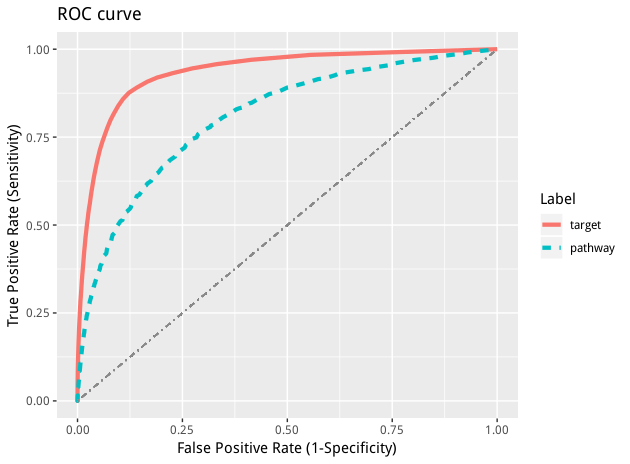
\includegraphics[scale=0.7]{figures/Fig1.png}%scale:表格縮放
    \caption{圖標題}
    \label{fig:fig_label}
\end{figure}


\begin{center}
\captionof{table}{表格名稱}
\label{table:combination}
\begin{tabular}{ p{3cm}p{2.5cm}p{2.5cm}p{2.5cm}p{2.5cm}p{2.5cm}p{2.5cm} } %col width
    \Xhline{1.3pt}
    \textbf{} & \textbf{Method1}  & \textbf{Method2} & \textbf{Method3} & \textbf{Method4}\\  %\textbf 粗體
    \Xhline{1.3pt}
        All AUC & 0.954±0.070 & 0.957±0.069 & 0.956±0.068 & \textbf{0.964±0.069}  \\
        Fold AUC & 0.947±0.019 & 0.943±0.033 & \textbf{0.948±0.019} & 0.941±0.036   \\
        Accuracy & 0.994 & 0.992 & 0.994 & 0.992   \\
        Precision & 0.329 & 0.251 & 0.342 & 0.262\\
        Recall & 0.207 & 0.292 & 0.204 & 0.277 \\
        F1-score & 0.254 & 0.270 & 0.256 & 0.269\\
        MCC & 0.296 & 0.333 & 0.306 & 0.330 \\
    \Xhline{1.3pt}
\end{tabular}
\end{center}



 \begin{center}
\captionof{table}{表格2}
\label{table:combination}
\resizebox{\textwidth}{25mm}{ %重新設定表格長寬 \resizebox{寬}{高}{表格}
\begin{tabular}{cccccc} %l(left),r(right),c(center)
    \Xhline{1.3pt}
    \textbf{} & \textbf{Assaf Gottlieb}  & \textbf{FeiWang} & \textbf{Yin-Ying Wang} & \textbf{Xujun Liang} & \textbf{Our Work}\\ 
    \Xhline{1.3pt}
        \textbf{Drug} & 593(Drug Bank) & 799 & 928 & 763 & 1080(Drug Bank)\\
        \textbf{Indication/disease} & 313(OMIM) & 719 & 608 & 681 & 1390(Disease Ontology)\\
        \textbf{Associated}  & 1933(OMIM) & 3250(Li and Lu) & CTD & Wang et al., 2014 & 13271(PharmacotherapyDB)\\
        \textbf{method} & logistic regression & logistic regression & PINA & sparse subspace learning & random walk\\
        \textbf{AUC} & 0.92±0.02(10-fold) & 0.864(10-fold) & 0.8969(5-fold) & 0.9178±0.0121(5-fold)& 0.946±0.023(5-fold) \\
        &  &  &  & & 0.948±0.019(10-fold) \\
    \Xhline{1.3pt}
\end{tabular}}
\end{center}



\begin{center}
\captionof{table}{表格3}
\label{table:combination}
\scalebox{0.9}{ %表格縮放
\begin{tabular}{ll} 
    \Xhline{1.3pt}
    \textbf{compound} & \textbf{pubchemID} \\ 
    \Xhline{1.3pt}
        epigallocatechin gallate (EGCG) & 65064\\
        caffeic acid (CA) &	689043\\
        gallic acid (GA) & 370\\
        catechin (C) & 73160\\
        epicatechin (EC) & 72276\\
        gallocatechin (GC) & 9882981\\
        epigallocatechin (EGC) & 72277\\
        catechin gallate (CG) &	6419835\\
        epicatechin gallate (ECG) &	107905\\
        gallocatechin gallate (GCG)	& 199472\\
    \Xhline{1.3pt}
\end{tabular}}
\end{center}


